\newpage
\subsection{Pumpenansteuerung}
\label{subsec:Detailkonzept_Pumpenansteuerung}

Die 12 Pumpen werden direkt über den Mikrokontroller via Digitalausgänge angesteuert. Da jedoch der Mikrokontroller nicht genügend Strom liefern kann, wird ein Logik-MOSFET eingesetzt. Bei dem MOSFET handelt es sich um einen IRLR8726 von Infineon. Mit diesem wurde schon in früheren Projekten gearbeitet, bei welchen sich dieser als zuverlässig herausstellte. Dieser MOSFET zeichnet sich durch einen geringen R$_{DSon}$ von 5.8m$\Omega$, eine kleine Gatekapazität von 15nC, einer V$_{DS}$ Breakdownvoltage von 30V und einer hohen Strombelastbarkeit von maximal 86A aus. Die Ansteuerung ist relativ simpel aufgebaut und kann in Abbildung \ref{fig:Pumpenansteuerung} begutachtet werden. 

\begin{figure}[h!]
\centering
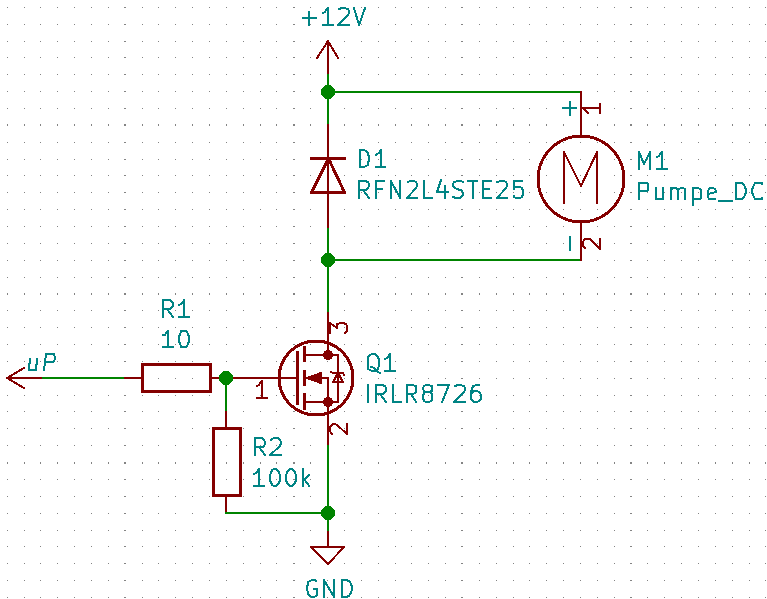
\includegraphics[width=0.6\textwidth]{graphics/Pumpenansteuerung.png}
\caption{Schema der Pumpenansteuerung}
\label{fig:Pumpenansteuerung}
\end{figure} 

Um den Gate-Eingang zu schonen, wird ein 10$\Omega$ Widerstand vogeschaltet. Parallel zur Pumpe ist eine Freilaufdiode verbaut, welche den Drain-Eingang der MOSFETS beim Ausschalten der Pumpe vor Spannungsspitzen schützt. 

\subsection{Durchflussmessgeräte}
\label{subsec:Detailkonzept_Durchflussmessgeräte}

Um die Durchflussmessgeräte ansteuern zu können, wird keine zusätzliche Elektronik benötigt. Es wird lediglich eine 5V Speisung sowie ein Analog- oder Digitaleingang eines Mikrocontrollers benötigt. Dabei wird jedoch ein Digitaleingang bevorzugt, da keine unterschiedlichen Spannungen eingelesen werden müssen, sondern lediglich High- und Lowpegel. Das Durchflussmessgerät sendet somit bei laufender Umdrehungszahl ein gepulstes Signal, welches mit steigendem Durchfluss die Frequenz erhöht. Dies geschieht bei gleichbleibendem Duty-Cycle von 50\%.